\documentclass[menu.tex]{subfiles}
\graphicspath{ {images/} }
\begin{document}    
    \begin{tabular} {p{3.5cm} p{4cm} p{9cm}}
        \multicolumn{3}{c}{\begin{LARGE}Menú Semanal 1\end{LARGE}}\\
        \hline
    
        %---LUNES---%
        \pbox{20cm}
        {
            \rule{0pt}{3ex}\begin{large}\textbf{Lunes}\end{large}\\ 
            \rule{0pt}{2ex}Atún con \\cebollines \\
            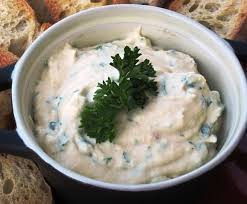
\includegraphics[scale=0.4]{atun-cebollines} 
        } & 
        \vspace{-2cm}
        \begin{compactitem} 
            \begin{footnotesize}
                \item 1/2 lata de atún
                \item 1 manojo de cebollin picado
                \item 1 manojo de perejil picado
                \item Mayonesa light
                \item Lechuga
            \end{footnotesize}
        \end{compactitem}&
        \vspace{-2cm}
        Mezcla media lata de atún al agua con los cebollines picados a gusto (recomendable una cantidad generosa). Agregar perejil picado a gusto (para un sabor potente se recomienda una buena cantidad) y mayonesa light. Mezclar todos los ingredientes, servir sobre una hoja de lechuga y acompañar con otros vegetales.\\
        \hline
        
        %---MARTES---%
        \pbox{20cm}
        {
            \rule{0pt}{3ex}\begin{large}\textbf{Martes}\end{large}\\
            \rule{0pt}{2ex}Albóndigas rellenas\\
            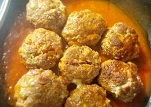
\includegraphics[scale=0.0092]{albondigas-rellenas}
        }&
        \vspace{-1.6cm}
        \begin{compactitem} 
            \begin{footnotesize}
                \item Albóndigas de res o atún
                \item Salvado de trigo
                \item Jamón
                \item Queso
                \item Huevo
            \end{footnotesize}
        \end{compactitem}&
        \vspace{-1.6cm}
        Prepare las albóndigas tal como sabe hacerlas, solo que, en vez de usar pan molido, utilice salvado de trigo o de avena muy bien molidos (si la marca que compro no viene bien molida, licue el salvado en seco hasta que se parezca a la harina). Haga un hueco en la albóndiga y rellene con queso y jamón picados en forma fina, cocinarlos en aceite. Aplane la preparación sin rellenar y tendrás unas agradables hamburguesas dietéticas. Use poco huevo para no requerir mucho salvado ya que este al ser cocidos tiende a endurecerse. Puede probar la misma preparación en base a atún al agua.\\
        \hline
        
        %---MIERCOLES---%
        \pbox{20cm}
        {
            \rule{0pt}{3ex}\begin{large}\textbf{Miércoles}\end{large}\\
            \rule{0pt}{2ex}Tacos en base de \\ tortillas y en base \\ vegetal \\ 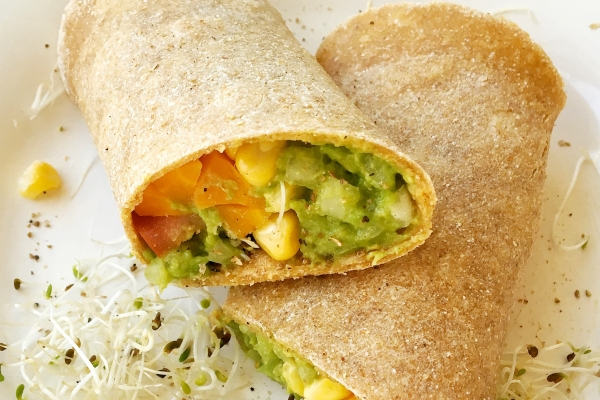
\includegraphics[scale=0.17]{tacos-integrales}
        }&
        \vspace{-2cm}
        \begin{compactitem} 
            \begin{footnotesize}
                \item Tortillas integrales o Lechuga
                \item Carne molida
                \item Tomate
                \item Cebolla
                \item Palta
            \end{footnotesize}
        \end{compactitem}&
        \vspace{-2cm}
        Sobre una tortilla integral coloque carne molida cocinada, vegetales, tomate, cebolla y un poco de palta. Puede preparar los tacos sobre 2 hojas grandes de lechuga, de este modo se reduce significativamente la cantidad de calorías.\\
        \hline
        
        %---JUEVES---%
        \pbox{20cm}
        {
            \rule{0pt}{3ex}\begin{large}\textbf{Jueves}\end{large}\\
            \rule{0pt}{2ex}Pastel de carote,\\ brócoli o berenjenas\\
            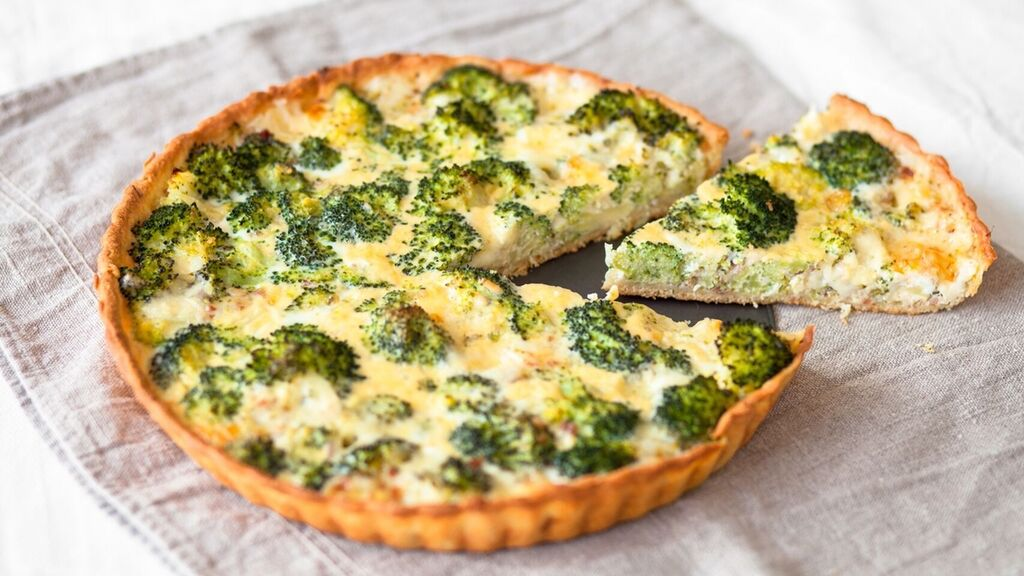
\includegraphics[scale=0.42]{pastel-brocoli}
        } & 
        \vspace{-1.6cm}
        \begin{compactitem} 
            \begin{footnotesize}
                \item Carotes o berenjenas o brócoli
                \item Huevo
                \item Jamón
                \item Queso
            \end{footnotesize}
        \end{compactitem}&
        \vspace{-1.6cm}
        Coloque en una bandeja una fila de carotes o berenjenas cortados en rodajas o brócoli cocido picado. Cubra esta capa con huevo, coloque jamón, vegetales y queso rallado. Cubra nuevamente con carotes, berenjenas o brócoli, De este modo coloque capas hasta formar un pastel del tamaño que le agrade y hornee.\\
        \hline
        
        %---VIERNES---%
        \pbox{20cm}
        {
            \rule{0pt}{3ex}\begin{large}\textbf{Viernes}\end{large}\\
            \rule{0pt}{2ex}Berenjenas rebozadas\\
            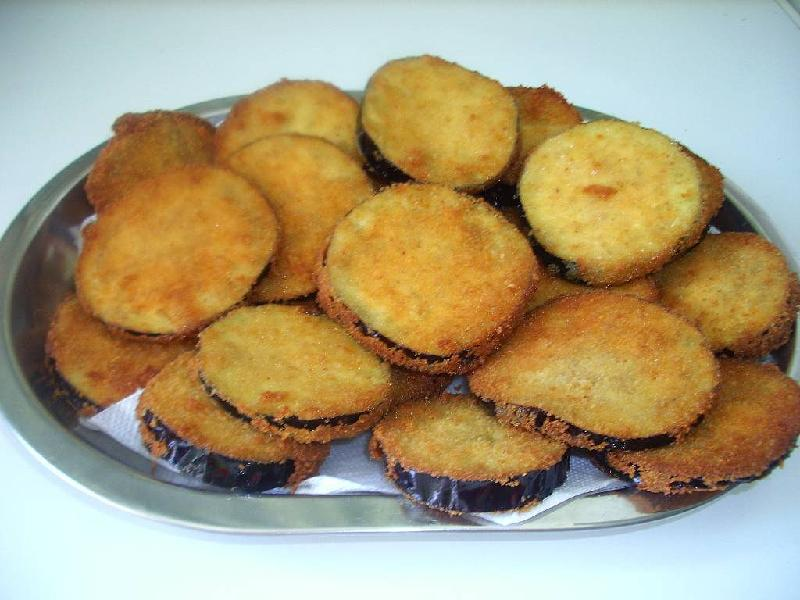
\includegraphics[scale=0.13]{berenjenas_rebozadas}
        } & 
        \vspace{-1.8cm}
        \begin{compactitem} 
            \begin{footnotesize}
                \item Berenjenas
                \item Huevo
                \item Sal
                \item Pimienta
                \item Aceite de oliva
            \end{footnotesize}
        \end{compactitem}&
        \vspace{-1.8cm}
        Corte las berenjenas en lonjas y úntelas en una preparación que incluya huevo, sal y una pizca de pimienta, cocínelas en un poco de aceite de oliva o en aerosol.\\
        \hline
        
        %---SABADO---%
        \pbox{20cm}
        {
            \rule{0pt}{3ex}\begin{large}\textbf{Sábado}\end{large}\\
            \rule{0pt}{2ex}Ensalada Cesar\\
            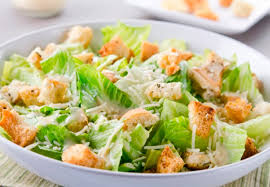
\includegraphics[scale=0.40]{ensalada-cesar}
        }& 
        \vspace{-1.6cm}
        \begin{compactitem} 
            \begin{footnotesize}
                \item Verduras
                \item Huevo
                \item Queso
                \item Jamon o enrollado de pollo
                \item Aceitunas
                \item Carne en trocitos de pollo
                \item Salsa cesar light
            \end{footnotesize}
        \end{compactitem}&
        \vspace{-1.6cm}
        Mezcle las verduras de su preferencia con huevos, queso en cuadrados, jamón o enrollado de pollo, aceitunas y carne en trocitos o pollo desmenuzado, coloque salsa cesar light (de cualquier marca) para decorar y sazonar. \\ \hline
\newpage
    \end{tabular}
    \end{document}
